\chapter{Genome Sequencing}
Genome sequencing is the process of determining a certain part or the complete DNA sequence of an organism's genome at a single time. Old biological techniques, that took into consideration small fragments of DNA for automatically sequencing, were not based on computation:
\begin{itemize}
	\item \textbf{Sanger sequencing} (\textit{Chain-Termination Method}): single stranded DNA molecules that differ in length by one nucleotide can be separated by polyacrylamide gel electrophoresis. Length ranging from 10 to 1500 nucleotides and the sequence can be read on the gel.
	\image{img/Sanger}{Sanger Technique.}{0.57}
	\item \textbf{PCR} (\textit{Polymerase Chain Reaction}).
	\image{img/PCR}{PCR Technique.}{0.9}
\end{itemize}

Sequencing a genome has an intrinsic complexity, for example, it is necessary to consider the degree of reliability of the obtained sequence. Repeated regions are mostly problematic, indeed, genomes may contain a lot of repeated sequences, for instance, in the Homo Sapiens genome, the repeated regions represent around the 35-50 \% of the total genome. For this reason, important questions are: Does the genome under the examination present repeated regions? What kind of repetitions? How long are these regions? What is the "degree of conservation" of the repeated regions?\\
When we talk about genome sequencing techniques, surely, we must consider the \textbf{shotgun sequencing} technique and its main variant the \textbf{double-barreled shotgun}. All sequencing projects consists in the following phases. After fragmenting and amplifying the DNA, for any DNA sequence obtained:
\begin{enumerate}
	\item DNA sequencing. (Biologist)
	\item Fragment-assembly. (Computer Scientist)
	\item Finishing. (Biologist)
\end{enumerate}

\section{Shotgun Sequencing}
Shotgun was developed in 1982 by Sanger and successively refined. It has three phases as can be seen in the following lines.
\subsection{Step 1 - DNA sequencing.}
It starts partitioning the DNA into sequences, suppose a length of 100.000 bp (\textit{base pairs}), and for each one apply the following steps:
\begin{enumerate}
	\item Produce a large number of copies of the source DNA (\textit{amplification}).
	\item Random fracture the sample, either using sound (\textit{sonication}) or passing it through a nozzle under pressure (\textit{nebulation}). The process produces a uniformly random partitioning of each copy of the source sequence into a collection of \textbf{DNA fragments}.
	\item Fragments that are too large or too small are removed, using gel electrophoresis. The band of gel containing the desired size is selected.
	\item The size-selected fragments are inserted in the DNA of genetically engineered bacterial virus (\textit{phage}), called \textbf{vectors}. Usually, one fragment is inserted into a vector at a predetermined point, called \textbf{cloning site}. The fragments are called \textbf{inserts} and the collection of fragments is called a \textbf{shotgun library}.
	\item A bacterium is infected with a single vector, which reproduces itself producing a bacterial colony containing million of copies (clones) of the vector and its associated insert. This procedure is repeated simultaneously for as many inserts as desired.
	\item By design, the vector permits a sequencing reaction (Sanger - chain termination method) to be performed, starting just at the fragment's insertion point. The sequencing reaction produces a read of the first 300-900 bases of one end of the insert.
\end{enumerate}
With these steps, a set of reads, randomly sampled from the source sequence is produced.
\image{img/DNAsequencing}{DNA Sequencing.}{0.8}
\paragraph*{Failure points: Bias.} A failure in the process may occur if the reads are not randomly sampled but biased to come from particular regions of the source DNA. This can happen for three reasons:
\begin{enumerate}
	\item The fracturing of the sample might be biased.
	\item The insertion of fragments into vectors might be biased.
	\item Some insert/vector combinations might not clone properly because the insert has reacted toxically with the host/vector environment.
\end{enumerate}
Practical evidence suggests that the first two biases are minimal in well-performed experiments, but the third bias definitely exists. Picking host/vector combinations for which the insert DNA will be relatively inert will reduce the toxicity bias.

\paragraph*{Failure points: Errors in reads.} Reads may contain errors for a variety of reasons: 
\begin{itemize}
	\item Technicians must screen the failed reads from vectors where no insert occurred.
	\item The sequencing reaction begins at one end of the insert location or at the other. The initial part of a read contain the vector sequence leading up to the beginning of the insert. This bit of vector sequence must be carefully removed.
	\item If an insert is short, technicians might need to trim the vector sequence from the end of a read.
\end{itemize}  

\subsection{Phase 2 - Fragment assembly}
Once all the reads of the shotgun library are available, the computational problem starts: it is necessary to arrange all the fragments to obtain the source DNA sequence. This is called \textbf{fragment-assembly problem}.
\image{img/fragmentAssembly}{Fragment-Assembly step.}{0.8}

\paragraph*{Redundancy and coverage.} The Number of sequenced (read) bases must be sufficiently high to ensure that all the genome has been covered. Now, it is important understand the meaning of some specific information that will be useful in the following pages:
\begin{itemize}
	\item \textbf{G:} length of the target sequence (genome size).
	\item \textbf{\textbf{F} = $\{f_1, f_2, \dots, f_R\}$:} set of reads.
	\item \textbf{L:} average length of a read.
	\item \textbf{R:} number of reads in shotgun dataset.
	\item \textbf{N = RL:} total number of base pairs sequenced.
\end{itemize}
The \textbf{average redundancy} or \textbf{coverage} is given by:
$$c = N/G ~ = ~ \text{number of sequenced bases}/\text{genome size}$$
For example suppose that 4 million bases of a bacterial genome have been sequenced and that the genome size is 4 Mb, then the coverage is 1x.\\
As genome coverage grows, the closure of regions not yet sequenced becomes highly probable. By using the Poisson distribution equation, it is possible to establish the probability $P_0$ that a base has not been sequenced, with respect to the coverage value $c$:
$$P_0 = e^{-c}$$
The percentage of effective coverage is:
$$\% Cov = 100 \cdot (1-e^{-c})$$
	\begin{figure}[H]
	\begin{minipage}[t]{0.45\linewidth}
		\centering
		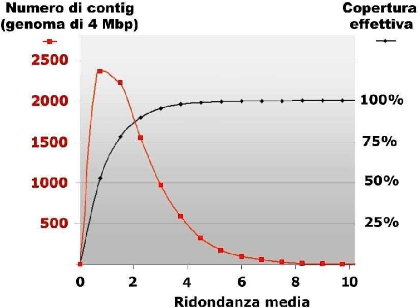
\includegraphics[width=\textwidth]{img/coverage}
		\caption{Coverage function.}
	\end{minipage}
	\hspace{1.8cm}
	\begin{minipage}[t]{0.42\linewidth} 
		\centering
		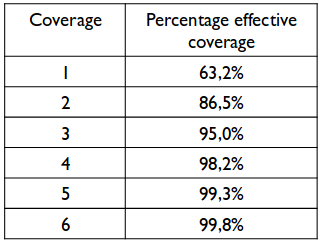
\includegraphics[width=\textwidth]{img/coverage_table}
		\caption{Percentage effective coverage.}
	\end{minipage}        
\end{figure}
\FloatBarrier
Usually a coverage of 10 is considered.

\paragraph*{Data peculiarities: bias and errors.} A computational solution of the fragment-assembly problem must consider the following data characteristics:
\begin{itemize}
	\item \textbf{Incomplete coverage:} not every bp of the sequence under examination is sequenced exactly $c$ times because of the stochastic nature of the process. The random steps might be biased and some parts of the sequence can be covered more than $c$ times, while other parts aren't covered at all.
	\item \textbf{Gaps:} are contiguous regions of maximal length that are not covered. Gaps lead to fragmented or incomplete solutions of the problem.
	\item \textbf{Sequencing errors:} the sequencing process of the inserts can cause errors which depend on the position in the insert ($<1\%$ for the first 500 bases; up to $15\%$ from 600 to 900 bases). Quality values can be associated to the bases in the reads. 
\end{itemize}

\paragraph*{Data peculiarities: orientation and repeats.} Other data features can be:
\begin{itemize}
	\item \textbf{Orientation:} the DNA is a double string. Only one end of the insert is sequenced. The right sequence to use might be either the read or its reversed 
	complement. Usually solved by sequencers.
	\item \textbf{Repeated sequences:} can cause assembly errors. In the picture the top represents the correct layout of three DNA sequences. The bottom shows a repeat collapsed in a misassembly.
\end{itemize}
\image{img/pec_orientation}{Repeated sequences.}{0.6}

\par \bigskip \noindent
Several computer science solutions are available when we consider the fragment-assembly steps:
\begin{itemize}
	\item \textbf{Exact approach:} \textit{shortest superstring problem} (SSP)
	\item \textbf{Heuristic (and greedy) approach:} \textit{Overlap-Layout-Consensus} (OLC), where:
	\begin{itemize}
		\item \textbf{Phase 1: overlap detection} (\textit{without errors}) $\rightarrow$ all pairs suffix-prefix matching.
		\item \textbf{Phase 1: overlap detection} (\textit{with errors}) $\rightarrow$ we can have also imperfect suffixes or prefixes composed by gaps/mismatches (\textit{semi-global alignment}) or matches that are not exactly suffixes or prefixes (\textit{LCS}). It has several implementations as: 
		\begin{itemize}
			\item \textbf{Semi-global alignment} (\textit{exact}): it is exact since it keeps only prefixes and suffixes but it can contain errors since there can be the presence of mismatches and gaps.
			\item \textbf{LCS}: Longest Common Substring problem (\textit{heuristic}). It keeps the longest common substring between two strings but this doesn't ensure the fact that the string is a suffix or a prefix, it could be also on the central part of the string.
			\item FASTA or BLAST (\textit{heuristic}).
		\end{itemize}
		\item \textbf{Phase 2: Fragment Layout} $\rightarrow$ a greedy approach.
		\item \textbf{Phase 3: Consensus} $\rightarrow$ by using multiple sequence analysis.
		\item \textbf{Graph-based OLC}
	\end{itemize}
\end{itemize}

\subsubsection{SSP - An exact approach}
A first approach is to formalize the problem in terms of a string problem, more precisely, the \textbf{shortest superstring problem} (\textit{SSP}). Given a set of strings $P=\{s_1, s_2, \dots, s_k\}$, a superstring of P is a single string that contains every string in P as a substring, for example, a concatenation of the strings of P in any order produces a superstring.\\
Given $P =\{\verb|abcc|, \verb|efab|, \verb|bccla| \}$ then "$\verb|bcclabccefab|$" and "$\verb|efabccla|$" are two superstrings of P. Moreover "$\verb|efabccla|$" is a shortest superstring.\\
Looking for the shortest superstring of P, strings in P are the reads and the shortest superstring containing all the strings in P is a good candidate for target DNA (parsimony assumption).\\
SSP has problem with repeats as can be seen in the following example considering the following sequence:
$$\verb|AATCTGGAGCTCT|$$
and its fragments:
\begin{enumerate}
	\item $\verb|AAT|$
	\item $\verb|CTGG|$
	\item $\verb|AGC|$
	\item $\verb|TCT|$
\end{enumerate}
The sequence can be obtained by simply concatenating the four fragments. However, the shortest substring of the set of fragments is:
$$\verb|AATCTGGAGC|$$
that collapses the repeated string "$\verb|TCT|$". The shortest substring problem is applied to fragment-assembly and data compression, it is an NP-Hard. For this reason heuristics to solve the SSP problem may be used, there are, indeed, polynomial algorithms which approximate the optimal solution of SSP within an arbitrary but predetermined constant.
Besides this, SSP have further problems in modeling the fragment-assembly such as:
\begin{enumerate}
	\item \textbf{SSP does not model possible read errors}. Errors might include:
	\begin{itemize}
		\item Insertion errors where a base is wrongly present in a fragment.
		\item Deletion errors where a base is absent from a fragment.
		\item Substitution errors where a base is substituted for another in a fragment. \item Chimeric errors where two disjoint fragments join to from a single non-existing fragment.
	\end{itemize}
	\item \textbf{SSP does not model fragment orientation}.
	\item \textbf{SSP fails in the presence of repeats}.
\end{enumerate}
For these reasons SSP is considered only of theoretical interest.

\subsubsection{OLC - An approximated approach}
OLC (Overlap-Layout-Consensus) is an approximate (heuristic) and greedy solution to the fragment-assembly problem, it consists of a three steps process:
\begin{itemize}
	\item Step 1: Overlap detection.
	\item Step 2: Fragment Layout.
	\item Step 3: Deciding the Consensus.
\end{itemize}

\paragraph*{OLC Step 1: Overlap detection (\textit{without errors}).} The problem consists of determining, for every ordered pair of reads, how much of the suffix of the first coincides with the prefix of the second. It should also consider their orientation.\\
In this specific case, without errors, for every ordered pair of strings $S_1$ and $S_2$, find the longest suffix of $S_1$ which is also a prefix of $S_2$ (\textit{suffix-prefix match problem}). Given two strings $S_1$ and $S_2$, any suffix of $S_1$ that matches a prefix of $S_2$ is called \textbf{suffix-prefix} of $S_1$ and $S_2$.
\begin{center}
	
\includegraphics[width=0.25\columnwidth]{img/OLC_1a}
\end{center}
Given a collection of strings $S=\{S_1, \dots, S_k\}$ of total length $m$, the all-pairs suffix-prefix problem is the problem of finding, for each ordered pair $S_i$ and $S_j$ in S, the longest suffix-prefix match of $S_i$ and $S_j$. The number of matches that will be done in order to retrieve the longest suffix-prefix is $k^2$.\\
An exact algorithm is based on the use of a \textbf{generalized suffix tree}. In a suffix tree a terminal edge is labelled with a string termination symbol (usually $\textdollar_i$). The algorithm consists of the following steps:
\begin{enumerate}
	\item Construct the generalized suffix-tree $T(S)$ for the $k$ strings of S (each one with its additional terminal symbol).
	\item Construct a list $L(v)$ for each internal node $v$. $L(v)$ contains index $i$ if and only if $v$ is incident with a terminal edge labelled \$$_i$ (the path-label of $v$ is a suffix of $S_i$). The list $L(v)$, for each internal node $v$, can be built in linear time during (or after) the construction of $T(S)$. Let us consider the path going from the root to the leaf $j$ representing the entire string $S_j$, the key observation is the following:
	\begin{itemize}
		\item If $v$ is a node on the path and index $i$ is in $L(v)$, then the path-label of $v$ is a suffix of $S_i$ that matches a prefix of $S_j$.
		\item So, for each index $i$, the deepest node $v$ on the path to leaf $j$ such that $i \in L(v)$ identifies the longest match between a suffix of $S_i$ and a prefix of $S_j$. The path-label of $v$ is the longest suffix-prefix match of $S_i$ and $S_j$.
		\item By one traversal from the root to leaf $j$, we can find the deepest nodes for all $1 \leq i \leq k~(i \neq j)$.
	\end{itemize}
	\item Collect all the suffix-prefix matches by traversing $T(S)$ in a depth-first manner and maintaining $k$ stacks (one for each string):
	\begin{itemize}
		\item When a node $v$ is reached, push $v$ onto the $i$-th stack, for each $i \in L(v)$.
		\item When a leaf representing the whole string $S_i$ is reached, scan the $k$ stacks and record, for each index $i$ the current top of the $i$-th stack. If the $i$-th stack is empty, then there's no overlap between $S_i$ and $S_j$.
		\item When the depth-first traversal backs up past node $v$, pop the top of each stack whose index is in $L(v)$.
	\end{itemize}
\end{enumerate}
All the $k^2$ longest suffix-prefix matches of S can be found in $O(m+k^2)$ time. Since $m$ is the size of the input and $k^2$ is the size of the output, the algorithm is time optimal. Note that:
\begin{itemize}
	\item $m$ = average read length $\times$ number of reads = $LR$
	\item $k$ = number of reads = $R$
\end{itemize}
Hence, $O(m+k^2) = O(L \cdot R + R^2)$ 

\paragraph*{OLC Step 1: Overlap detection (\textit{with errors}).} The all-pair suffix-prefix matching solve the problem under the hypothesis that the sequenced data have no errors, but \textbf{sequencing errors exist}. For this reason, the suffix-prefix matching must admit approximations. The problem is to find a suffix $S_1$ and a prefix $S_2$ whose similarity is maximum over all suffix-prefix pairs of $S_1$ and $S_2$.\\
First of all, it is important to define the concept of similarity:
\begin{itemize}
	\item Positive matches make a positive contribution to the objective function.
	\item Mismatches and gaps make a negative contribution.
\end{itemize}
The most useful weights and penalties must be fixed. From another point of view, it can be seen as a \textbf{semi-global alignment} problem, indeed, a \textbf{variant of the Needleman-Wunsch} global alignment algorithm is considered (optimal alignment by admitting initial and final gaps without penalties).\\
Given two strings $x$ and $y$ of length $n$ and $m$, the inductive definition is:
\image{img/NW-OLC}{A variant of the NW algorithm}{0.7}
The maximum score is on the last row and/or column and the aligned string can be found by following the backward pointers until one element of the first row or column is reached.\\
For example, consider the Nucleotide similarity score matrix:
\image{img/similarity_score_matrix}{Similarity score matrix}{0.25}
and fix the gap penalty $d=2$.\\
By using the given recursive equation, we want to apply the algorithm to the strings:
\begin{enumerate}
	\item $x = \verb|GCCATCT|$
	\item $y = \verb|TCTAAGC|$
\end{enumerate}
The resulting table is:
\image{img/example_table}{Example of the variant of N-W algorithm.}{0.7}
If we take into consideration the complexity of this algorithm, we know that N-W algorithm is $\theta(nm)$, considering $n \simeq m$ and equal to $L$ (average length of a read), the complexity can be indicated as $\theta(L^2)$.\\
Let $R$ be the total number of reads, then the complexity of the overlap detection phase is $\theta(R^2L^2)$. Usually $L=400\text{ or }500$ and the number of reads $R$ is very high. Hence, the overlap detection is computationally very expensive and creates a bottleneck for the fragment-assembly problem, then, instead of an exact solution, heuristic solutions can be adopted. Heuristics for overlap detection try to find ordered pairs of strings with large similarity, for instance, two strings having a sufficiently long common substring are probably overlapping substrings. The corresponding computational problem is the \textbf{longest common substring} problem (\textit{LCS}), that can be efficiently solved using a generalized suffix tree.

\paragraph*{Longest Common Substring (LCS).} This algorithm is related to the problem that starting from two strings $S_1$ and $S_2$, it is needed to find the longest common substring. An exact solution is based on the construction of the generalized suffix-tree of $S_1$ and $S_2$ in which:
\begin{itemize}
	\item The leafs represent a suffix of $S_1$ or $S_2$.
	\item Each internal node $v$ is marked with 1 and/or 2 if and only if there is a leaf in the subtree of root $v$ that is a suffix of $S_1$ and/or $S_2$.
	\item Internal nodes marked both 1 and 2 correspond to common substrings of $S_1$ and $S_2$. The longest of such substrings is the solution to the problem.
\end{itemize}
The algorithm must find the node which is marked 1 and 2 and with the \textbf{greater string-depth} (number of characters in the path from the root to the node). The algorithm steps are the following:
\begin{enumerate}
	\item Build the generalized suffix-tree for $S_1$ and $S_2$.
	\item Mark the internal nodes and compute their string-depth.
	\item Return the substring with maximal string-depth which corresponds to a node marked both 1 and 2.
\end{enumerate}
The first step requires linear time with respect to the sum of the lengths of $S_1$ and $S_2$, also the further steps can be performed in linear time by tree traversal.\\
The LCS problem is only an heuristic for the overlap detection phase and for this reason it could not bring us to an optimal solution. For example:
\begin{center}
	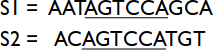
\includegraphics[width=0.22\columnwidth]{img/LCS_example}
\end{center}
The longest common substring is underlined but we can suppose the fact that it could be a repeat, then the two strings may not be overlapping or the fact that this procedure doesn't allow for errors.

\paragraph*{Further Heuristics.} Other heuristics use BLAST or FASTA to find a good local alignment among all possible pairs of strings. The higher the score, the greater the probability that the two corresponding strings are overlapping.\\
These techniques greatly reduce the overall computation time for sequence-assembly. They allow for errors in the reads.

\paragraph*{OLC Step 2: Fragment Layout - Greedy solution.} In this phase one tries to rebuild the target DNA sequence by using the overlaps. There are various approaches to this problem. The first (and most practical) implementations follow some variant of the following greedy approach:
\begin{itemize}
	\item The string pair with highest suffix-prefix (or overlapping) score is chosen and merged. This step forms the \textbf{first contig} (set of contiguous DNA segments):
	\begin{center}
		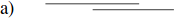
\includegraphics[width=0.22\columnwidth]{img/contigA}
	\end{center}
	\item Then, the next highest score pair is selected and merged, resulting either in one contig containing three strings (\textit{b}) or in two separate contigs containing four strings (\textit{c}):
	\begin{center}
		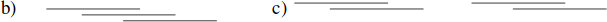
\includegraphics[width=0.8\columnwidth]{img/contigBC}
	\end{center}
	\item Iterate. 
\end{itemize} 
Since the suffix-prefix overlaps are determined by similarity criteria, gaps are allowed in the suffix-prefix matches. As successive inserts are added into a contig, additional gaps may have to be inserted into the added string to be consistent with gaps in the previously inserted strings.\\
The main difficulty in this phase is to decide whether two fragments with a good overlapping score:
\begin{itemize}
	\item \textbf{Do effectively overlap} (hence their differences are due to sequencing errors).
	\item Or \textbf{represent a repeat} in the genome (hence their differences are due to mutations).
\end{itemize}

\paragraph*{OLC Step 3: Consensus.} In this phase we must determine the consensus on each contig. For each position of a contig it may happen that:
\begin{itemize}
	\item All characters coincide: no problem for that position.
	\item There is a disagreement in the aligned characters in that position: a choice has to be made.
\end{itemize}
Various approaches to obtain the consensus sequence:
\begin{itemize}
	\item The simplest one reports the frequency of each character at each position (\textit{profile}) and let the user decide how to use that information.
	\item Alternatively a consensus sequence can be obtained by taking the plurality of characters on each position, provided the plurality is above some preset threshold.
\end{itemize}

\paragraph*{OLC: A general overview.} The OLC assemblers discussed so far are called \textbf{greedy assemblers} because they employ greedy algorithms in the layout phase. The greedy algorithms apply one basic operation: given any read or contig, add one more read or contig, this basic operation is repeated until no more operations are possible. Each operation uses the next highest-scoring overlap to make the next join. The scoring function measures, for instance, the number of matching bases in the overlap, thus the contigs grow by greedy extension, always taking on the read that is found by following the highest-scoring overlap.\\
However, greedy assemblers have also the following problems:
\begin{enumerate}
	\item The greedy algorithms can get stuck at \textbf{local maxima}.
	\item Overlaps induced by repetitive sequences may score higher than real overlaps.
	\item The greedy algorithms need mechanisms to avoid incorporating false-positive overlaps into contigs.
	\item An assembler that builds on false-positive overlaps will join unrelated sequences and produce \textbf{chimera}.
\end{enumerate}

\paragraph*{Graph-based OLC.} OLC assemblers can be also graph-based, they use the so-called \textbf{overlap graph}. An overlap graph represents the reads and their overlaps:
\begin{itemize}
	\item Nodes represent the reads.
	\item Edges represent overlaps.
\end{itemize}
The graph-based OLC approach consists of three phases:
\begin{enumerate}
	\item \textbf{Overlap:} overlap detection using one of the already discussed techniques.
	\item \textbf{Layout:} construction and manipulation of an overlap graph, paths in the graphs are potential contigs. The overlap graph does not represent single bases, so large-genome graphs may fit into computer memory.
	\item \textbf{Consensus:} a multiple sequence alignment (MSA) determines the layout and then the consensus sequence. Heuristics are generally used for MSA. The consensus phase must load the sequences of bases into memory.
\end{enumerate}
For instance, suppose to have three copies of an unknown target DNA sequence:
\begin{center}
	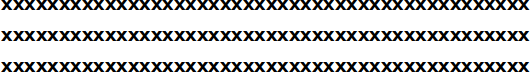
\includegraphics[width=0.8\columnwidth]{img/example_graphOLC}
\end{center}
Suppose the obtained reads are: \verb|accgt|, \verb|aggt|, \verb|acgatac|, \verb|accttta|, \verb|tttaac|, \verb|gataca|, \verb|accgtacc|, \verb|ggt|, \verb|acaggt|, \verb|taacgat|, \verb|accg|,\verb|tacctt|.
\begin{itemize}
	\item The first step is the overlap detection among reads.
	\item The second step is the construction of a graph whose nodes represent reads and edges indicate overlaps between reads.
	\image{img/OLC_exampleGraph}{Example of a graph-based OLC.}{0.65}
	\item The third step consists in refining the graph by detecting the transitive edges and solving the ambiguities. The output of this step is a set of simple paths with no intersections, each one corresponding to a contig. The consensus sequence is obtained by performing a multiple alignment (MSA) of the reads which compose the path under examination.\\
	In our example we obtain a single path: \verb|accgtacctttaacgatacaggt|. This is a very simple case in which no errors, no repetitions and a little coverage is present.
\end{itemize}



\subsection{Phase 3 - Finishing}
Imperfect coverage, repeats, and sequencing errors cause the assembler to produce not one, but hundreds or even thousands of contigs. The task of closing gaps between contigs and obtaining one complete sequence is called \textbf{finishing}.
\image{img/finishing}{Finishing procedure.}{0.8}
A process called \textbf{scaffolding} is used to order and orient the contigs with respect to each other into larger structures called \textbf{scaffolds}. A scaffold is a maximally linked and ordered set of contigs.\\
In this phase it is possible to distinguish two types of gaps:
\begin{itemize}
	\item The gaps between contigs belonging to the same scaffold are called \textbf{sequence gaps}. They represent genuine gaps in the sequence.
	\item The gaps between scaffolds are called \textbf{physical gaps} because the physical DNA that would span them is either not present in the clone inserts or indeterminable due to misassemblies. Filling these gaps is more difficult and it involves a large amount of manual labor and complex laboratory techniques. 
\end{itemize}

\section{Double-barreled shotgun sequencing}
It is a main variant of the shotgun sequencing: the inserts average length, $l$, is longer than $2L$ and both ends of the insert are sequenced.\\
This procedure gives rise to a pair of reads, called \textbf{mates}, that are in opposite orientation and at a distance from each other approximately equal to $l$ (the insert average length).\\
The main difference with the shotgun sequencing is the fact that in this case we take into consideration information that are both in the left and the right bound. In this way it is possible to reconstruct the sequence from both sides.
\image{img/doubleShotgun}{Double-barreled shotgun sequencing schema.}{0.8}
Once contigs are built, they must be oriented and joined and clone mate information is relevant for this.
\image{img/doubleShotgun2}{Mates are useful for scaffolding.}{0.8}
A \textbf{scaffold} is a maximally linked and ordered set of contigs.
\image{img/doubleShotgun3}{Scaffolding: contigs order.}{0.7}
The mate pairing information can be used for:
\begin{itemize}
	\item \textbf{Ordering contigs:}
		\begin{enumerate}
			\item If a read in a contig has its mate in another contig, then we can suppose (by knowing the average length $l$ of the inserts) that the two contigs are adjacent.
			\item There should be various mate pairs in two possibly adjacent contigs, if their number (coverage) gives sufficient support, we can order contigs with a good reliability.
		\end{enumerate}
	\item \textbf{Identifying repeats:} the probability that both reads of an insert fall into the same repeat is low. This depend on $l$ and on the size of the repeat.
\end{itemize}
In order to build a scaffold, it is essential to create a graph whose nodes are contigs and an edge links two nodes when mate pairs bridge the gap. This lead to have computational problems as finding all the connected components in the graph, finding a consistent orientation for all nodes and embedding the graph in a sequence respecting estimates on edge lengths.\\
\textbf{Sequence gaps} are gaps in the clone which can be resequenced by PCR. \textbf{Physical gaps} are, instead, gaps between scaffolds. They corresponds to parts of DNA not present in the clones (not in the library). Mates can be used also to distinguish the two cases. 
\image{img/doubleShotgun4}{Scaffolding gaps.}{0.7}

\section{Techniques used for sequencing human genome}
Three different strategies have been used for sequencing the human genome:
\begin{itemize}
	\item Hierarchical sequencing used by HGP. This method is also called clone-by-clone sequencing or BAC-by-BAC sequencing.
	\item Sequence-tagged connector approach (\textit{a variant of hierarchical sequencing})
	\item Whole-genome shotgun sequencing used by Celera Genomics.
\end{itemize}

\subsection{Hierarchical sequencing}
The hierarchical sequencing approach can be sum up with the help of the following image:
\image{img/hierarchical}{Hierarchical sequencing.}{0.7}
The algorithm is subdivided in the following steps:
\begin{enumerate}
	\item Creation of a BAC library: random fragmentation of the genome into sequences of 50-300 kbp length, then inserted into BACs (Bacterial Artificial Chromosomes).
	\item Determining an assembly or \textbf{physical map}.
		\begin{center}
			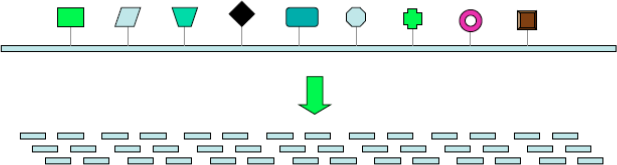
\includegraphics[width=0.8\columnwidth]{img/hierarchical3}
		\end{center}
		A map of the genome may be useful to order the fragments. A physical map is given by a set of markers (often genes or known patterns, such as enzymes or specific proteins) in the genome. The metric used is based on observable or countable physical features, usually the number of nucleotides between two points. The physical map must be accurate: error in this phase could produce "chimera" chromosomes.
	\item Determining a minimal tiling path of BACs that covers the genome, that is a set of clones with minimal overlapping. Overlaps between BAC inserts are determined on the basis of fingerprint data on each insert.
	\item Shotgun sequencing of each tiling clone.
	\item Finishing phase.
		\begin{center}
			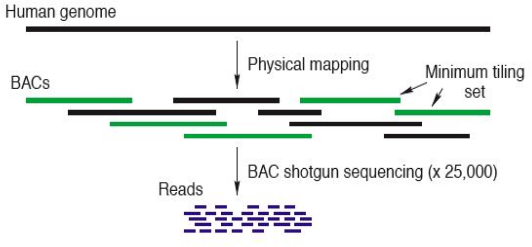
\includegraphics[width=0.8\columnwidth]{img/hierarchical2}
		\end{center}
\end{enumerate}
The clone-by-clone technique requires two separates processes: \textbf{sequencing} and \textbf{physical mapping}. The first one is heavily automated, while the second one requires a lot of hand working.\\
Physical maps are difficult and time consuming to build, on the other hand, they are useful for studying specific genome sectors and allow for a scalable approach. Moreover they ease the finishing phase.

\subsection{Sequenced-tagged connector approach}
A variant of the hierarchical approach which avoids the building of a physical map. It consists on the following steps:
\begin{enumerate}
	\item A library BACs is sequenced (600.000 for the human genome).
	\item A set of seed BACs are randomly selected. They are used for an ordered clone-by-clone walk on the genome. 
	\item Each seed BAC is sequenced using the shotgun approach.
	\item Look for the overlapping BAC (using the end-sequence information) in both directions.
	\item Shotgun sequencing of the minimally overlapping BACs in both directions.
\end{enumerate}
\image{img/sequence-tagged}{Sequence-tagged connector approach.}{0.75}

\subsection{Whole-genome shotgun sequencing}
Apply the double-barreled shotgun sequencing with vectors of different size. The different size of the inserts and the mate-pairs information are used by heuristics to resolve the repeated sequences. Read completely interior to a repeat have the repeat's color, they are anchored, namely their mate is not in a repeat.
\image{img/whole-genome}{Whole-genome shotgun sequencing.}{0.8}

\subsection{Shotgun and variants: closing remarks}
As we said, a sequencing projects consist of the following phases:
\begin{enumerate}
	\item DNA sequencing (Biologist) $\rightarrow$ \textbf{Sanger chain termination method}
	\item Fragment-assembly (Computer Scientist)
	\item Finishing
\end{enumerate}
Using the Sanger sequencing technique for determining the reads implies:
\begin{itemize}
	\item \textbf{Pros:} well established and highly automated procedure, high accuracy.
	\item \textbf{Cons:} a single sequence per reaction is produced. Less than 1000 bases per read.
\end{itemize}

\section{SBH: Sequencing by Hybridisation}
SBH is an alternative to sequencing methods by electrophoresis, such as the Sanger method. SBH is based on DNA array or DNA chip, that are matrices containing synthetic probes of DNA. The approach works as follows:
\begin{enumerate}
	\item Attach all possible DNA probes of length $k$ to the matrix surface, each probe is at a distinct and known location. This set of probes is called \textbf{DNA array}.
	\item Apply a solution containing single-stranded fluorescently labelled DNA fragments to the array.
	\item The DNA fragments hybridises (bind) with probes that are complementary to substrings of length $k$ of the fragment.
	\item Using a spectroscope detector, detect all probes hybridising with the DNA fragment and obtain the set $S$ of $k$-mers (spectrum) of the DNA fragment.
	\item Reconstruct the sequence of the DNA fragment from the spectrum $S$ (Computer science step).
\end{enumerate}
It is an advantage to take $k$ as large as possible. In the first SBH proposed $k$ was 8, the "all 8-mers" DNA array requires synthesising $4^8 = 65536$ probes. Now $k$ can be 30 or greater.\\
Note that the step 5 can be modeled as a particular case of the shortest superstring problem (SSP) where all strings have constant length $k$.
\image{img/SBH1}{SBH with $k=5$.}{1}
\image{img/SBH2}{Example of SBH application with $k=3$.}{0.9}

\paragraph*{Graph of k-mers.} Given the spectrum $S$, it is possible to build the graph of the k-mers with overlapping, $H=(V_H, E_H): V_H = S$.\\
$E_H = \{(u,v): u,v \in S$ and the $(k-1)$-suffix of $u$ is equal to the $(k-1)$-prefix of $v\}$.
\image{img/SBH3}{Example of a graph of k-mers.}{0.8}

\paragraph*{Hamiltonian path.} A Hamiltonian path is a path that visits each vertex exactly once. 
\image{img/HamiltonianCycle}{Example of a Hamiltonian cycle.}{0.3}
A Hamiltonian path visiting all the vertices of $H$ is a solution of the SBH problem that is the target DNA sequence.\\
In the previous example the unique Hamiltonian path on graph $H$ produces the sequence $\verb|ATGTGCCGCA|$, which is exactly the target sequence. However, in the general case, the Hamiltonian path problem is NP-complete.

\paragraph*{Eulerian path (dual).} An Eulerian path is a path which visits every edge exactly once. For instance, in the next image, following the edges of this graph in alphabetical order gives a Eulerian cycle.
\begin{center}
	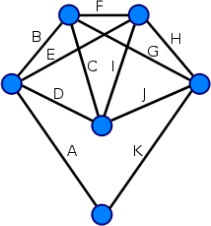
\includegraphics[width=0.3\columnwidth]{img/eulerian}
\end{center} 
We can transform the graph $H$ into a new graph $G$ (\textbf{De Bruijn graph}) in order to reduce the Hamiltonian path problem into the Eulerian path problem, which can be solved in \textbf{polynomial time}.

\paragraph*{De Bruijn graph G (dual of the graph of k-mers H).} A new graph $G$ is obtained from $H$ as follows:
\begin{itemize}
	\item $V_G$: set of all $(k-1)$-mers. Each k-mer of $H$ produces two $(k-1)$-mers in $G$, a prefix and a suffix.\\
	Example: $\verb|AAC|$ produces $\verb|AA|$ and $\verb|AC|$.
	\item $E_G$: an edge from node $u$ to node $v$ is in $G$ if and only if there exists a $k$-mer in $H$ containing $u$ as prefix and $v$ as suffix. Edges of $G$ represent $k$-mers, then an Eulerian path visiting each edge in $G$ exactly once gives a solution to the SBH problem.
\end{itemize}
Graph $G$ is called a \textbf{De Bruijn graph} (\textit{Euler graph}). Following our previous example:
\image{img/DeBruijn}{Example with Hamiltonian path and De Bruijn graph.}{0.8}
The unique Eulerian path of graph $G$ produces the sequence: $\verb|ATGTGCCGCA|$.\\
A possible problem that can be found is the fact that there can be more than one Eulerian path in the graph $G$. For example, considering the $3$-mers $\{\verb|ACT|, \verb|CTA|, \verb|TAC|\}$. We have two graphs:
\begin{center}
	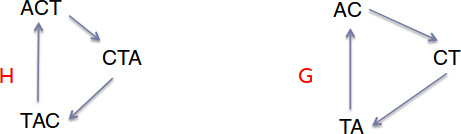
\includegraphics[width=0.7\columnwidth]{img/DeBruijn2}
\end{center} 
We can obtain three different sequences: $\verb|ACTAC|, \verb|TACTA| \text{ and } \verb|CTACT|$.\\
Each Eulerian path corresponds to a different DNA sequence, we can infer the sequence unambiguously if and only if the number of Eulerian paths in $G$ is exactly one.\\
Graph theory can supply:
\begin{itemize}
	\item Necessary and sufficient conditions for the existence of a Eulerian path in a graph.
	\item Necessary and sufficient conditions for the existence of a unique Eulerian path.
	\item Efficient algorithms for finding Eulerian paths in a graph.
\end{itemize}
SBH data contain errors caused by:
\begin{itemize}
	\item Hybridisation errors.
	\item Multiplicity errors.
\end{itemize}
Hybridisation errors give rise to:
\begin{itemize}
	\item \textbf{False negatives}: a k-mer appears in the sequence, but not in $H$.
	\item \textbf{False positives}: a k-mer does not appear in the sequence, but it is in $H$.
\end{itemize}

\section{De Bruijn graphs for assembly}
In 1995 it was proposed to use De Bruijn graphs for sequence assembly in the shotgun approach. The approach is usually called \textbf{De Bruijn approach}. The idea consists in decomposing each read of length $n$ into a set of $k$-mers: in a read of length $n$ there are $n-k+1$-mers.\\
Let $F=\{f_1, f_2, \dots, f_R\}$ be the set of reads. The \textbf{spectrum} is the set of all $k$-mers $w$ $(k=20,30)$:
$$\{(w,(i,i_{\alpha})) ~|~ w \in f_i, 1 \leq i \leq R\}$$
It means that $w$ occurs in read $f_i$ at position $i_{\alpha}$. The $k$-mer $w$ occurs $n(w)$ times in $F$ (\textit{coverage information}).
The De Bruijn approach follows these steps:
\begin{enumerate}
	\item Build the De Bruijn graph on the $k-1$-mers reporting on each edge the pair (read, position).
	\item Simplify the graph.
	\item Perform some variant of the Eulerian path to infer the sequences.
\end{enumerate}
It works well even in presence of errors. Reads with perfect overlaps induce a common path (a contig). Perfect overlaps are detected implicitly without any pairwise sequence alignment calculation.
\begin{center}
	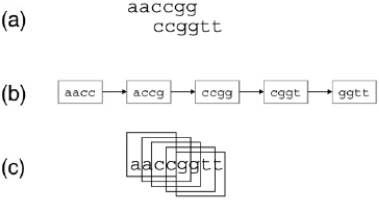
\includegraphics[width=0.7\columnwidth]{img/DeBruijn3}
\end{center} 
The pairwise alignment of the two reads in picture (\textit{a}) is a by-product of the graph construction (\textit{b}). The simple path through the graph implies a contig (\textit{c}).\\
Real sequencing data produce problems in overlap graphs and $k$-mer graphs:
\begin{itemize}
	\item \textbf{Spurs} are short, dead-end divergences from the main path. They are produced by sequencing error toward one end of a read. The error can be signalled by coverage dropping to zero.
	\begin{center}
		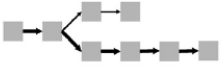
\includegraphics[width=0.4\columnwidth]{img/spurs}
	\end{center} 
	\item \textbf{Bubbles} are paths that diverge and then converge. They are produced by sequencing error toward the middle of a read, and by polymorphism in the target DNA. Efficient bubble detection is non-trivial.
	\begin{center}
		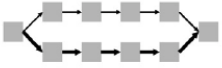
\includegraphics[width=0.4\columnwidth]{img/bubbles}
	\end{center} 
	\item Paths that converge and then diverge from the \textbf{frayed rope pattern}. They are produced by repeats in the target DNA.
	\begin{center}
		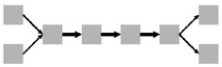
\includegraphics[width=0.4\columnwidth]{img/fragment}
	\end{center} 
	\item \textbf{Cycles} are paths that converge on themselves. They are produced by repeats in the target DNA. Through the associated info and number of occurrences of $k$-mers, it is possible to solve them.
\end{itemize}
All the described situations can occur together, creating a very complex graph structure.\\
Repetitions of a $k$-mer can occur:
\begin{itemize}
	\item \textbf{Within a single fragment in different locations (close):} when building the Eulerian path we make sure that edges corresponding to adjacent positions are visited successively. Moreover we can modify the Eulerian path construction by allowing multiple visits to the edges corresponding to repetitions.
	\item \textbf{As a repetitive regione in different fragmets (distant):} in this case the corresponding edge contains significantly more fragment positions than its non-repetitive neighbors.
\end{itemize} 
\paragraph*{De Bruijn approach: example.} Let's consider the sequence:
\begin{center}
	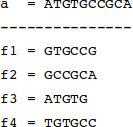
\includegraphics[width=0.2\columnwidth]{img/exampledeb}
\end{center} 
In this example we don't consider the complementary reads. For $K=3$ we have:
\begin{center}
	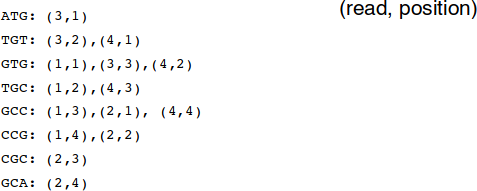
\includegraphics[width=0.8\columnwidth]{img/exampledeb2}
\end{center}
The corresponding Eulerian graph is:
\begin{center}
	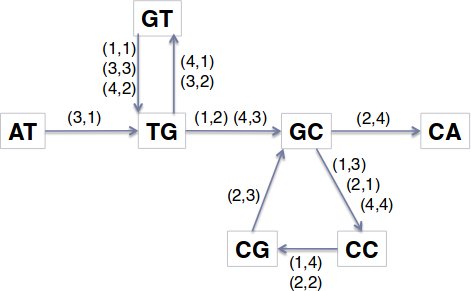
\includegraphics[width=0.7\columnwidth]{img/exampledeb3}
\end{center}

\section{Next Generation Sequencing}
New sequencing techniques have been developed, they allow for sequencing many DNA fragments in parallel, the new technologies are called \textbf{Next Generation Sequencing}. To sum up the improvement of this new technique we can see to these data:
\begin{itemize}
	\item \textbf{Sanger:} 1000bp, 100 reactions in parallel. Ten runs: 1 Mb.
	\item \textbf{NGS:} 50-500bp, millions of sequences in parallel. One run: 0,5-10 Gb.
\end{itemize}
NGS has an high throughput and a low cost, but on the other hand, it has less accuracy (less than 500 bp per read).\\
NGS has no need of cloning by means of virus or bacteria, no need of gel electrophoresis to discover the sequence of nucleotides. Sequencing is done step-by-step (pyrosequencing, sequencing by synthesis).

\paragraph*{Pyrosequencing.} Sequencing is performed by detecting each nucleotide incorporated by a DNA polymerase during DNA elongation. It relies on \textbf{light detection} each time a nucleotide is added.
\image{img/pyrosequencing}{Pyrosequencing approach.}{0.8}

\section{Sequencing Software}
Phred allows for assessing the quality of a DNA sequence on the basis of its electropherogram and by using statistical techniques. It compares the peaks and curves of sequenced fragments with the runs of well known sequences. It associate a quality value to each base.
\image{img/phread}{Phred execution.}{0.6}
Phred-score is the reliability value produced by Phred.

\section{Genome annotation}
With \textbf{genome annotation} we consider the fact of assigning identities and functions to sequences within the genome.\\
After sequencing there is the annotation phase, it requires many integrated tools for analysis and visualization of the sequenced genome. A main step is \textbf{gene inference}, it can happen through:
\begin{itemize}
	\item \textbf{Intrisic techniques:} protein-coding genes have recognizable features, there are several softwares to scan the genome and identify these features.
	\item \textbf{Estrinsic techniques:} comparison with known genomes and genes in other organisms.
	\item \textbf{Transcriptome analysis (RNA-seq):} an RNA sequence mirrors the sequence of the DNA from which it was transcribed. Consequently, by analyzing the entire collection of RNA sequences in a cell (\textit{transcriptome}), it is possible to determine when and where each gene is turned on or off in the cells and tissues of an organism. \textbf{RNA-seq} allows to quantify, discover and profile RNAs. 
\end{itemize}